\section{tun\_hdr\_t}\label{sec:tunhdr}

\begin{figure}
\begin{center}
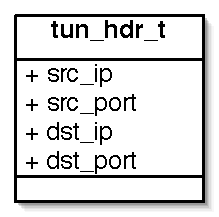
\includegraphics[width=0.4\textwidth]{figs/tunhdr}
\end{center}
\caption{}
\label{fig:tunhdr}
\end{figure}

This section describes the tun\_hdr\_t struct, which is described by Figure~\ref{fig:tunhdr}.  This component is a very simple data
structure that defines a single header needed to encapsulate a single layer of a NAT3 tunnel.  For example, with a single NAT box, 2
tun\_hdr\_t structures are needed (one for the outermost IP header, and one for the internal header).


\subsection{Member Variables}

\begin{itemize}
\item m\_uSrcIP: uint32\_t
\item m\_uSrcPort: uint16\_t
\item m\_uDstIP: uint32\_t
\item m\_uDstPort: uint16\_t
\end{itemize}

